% Source - https://tex.stackexchange.com/a/213415
% Posted by Christian Feuersänger, modified by community. See post 'Timeline' for change history
% Retrieved 2026-02-26, License - CC BY-SA 3.0

\documentclass{standalone}

\usepackage{pgfplots}
\pgfplotsset{compat=1.11}

\begin{document}
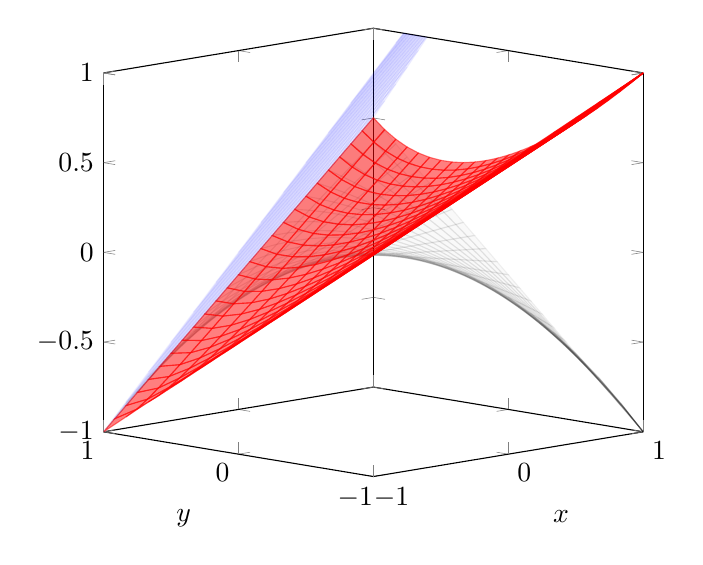
\begin{tikzpicture}
\begin{axis}[xlabel=$x$,ylabel=$y$,
    view={-45}{10},
    zmin=-1,zmax=1,
    variable=s,
    variable y=t,
    domain=0:1,
]
\def\triangleParamX{-1+ 2*s}
\def\triangleParamY{-1+ 2*(1-s)*t}
\addplot3[surf,color=gray,faceted color=black,opacity=0.05] (\triangleParamX,\triangleParamY,x*y);
\addplot3[surf,color=red,faceted color=red,opacity=0.5] (\triangleParamX,\triangleParamY,{(2*x*x+2*x+2*y*y-2*y)/(2*x-2*y+4)});
\addplot3[surf,color=blue,faceted color=blue,opacity=0.05] (\triangleParamX,\triangleParamY,{x-y+1});
\end{axis}
\end{tikzpicture}
\end{document}
